\documentclass[10pt,a4paper]{article}
\usepackage[utf8]{inputenc}
\usepackage{amsmath}
\usepackage{amsfonts}
\usepackage{amssymb}
\usepackage{array}
\usepackage{graphicx}
\graphicspath{ {images/} }
\author{Team V}
\title{GRN FanZone Requirements Document}

\begin{document}
\maketitle

\begin{center}
	\begin{tabular}{ |c|c|c| }
	\hline
	Revision & Author & Date \\ 
	\hline
	0.1 & Andrew McCluskey & 11/11/2016 \\
	\hline
	0.2 & Andrew McCluskey & 18/11/2016 \\
	\hline
	& & \\
	\hline
	& & \\
	\hline
	\end{tabular}
\end{center}

\newpage
\tableofcontents
\newpage

\section{Introduction}

\subsection{Purpose}
The purpose of the GRN FanZone is to provide fans of amateur to semi-professional rugby with a platform on which to interact with teams, clubs or players. GRN supports local rugby communities globally, giving them the tools to grow their quality of communication and reach; while having a user-friendly platform for all connections in one place.

\subsection{Definitions}

\begin{tabular}{ |l|l| }
\hline
GRN & The Global Rugby Network \\ 
\hline
Team V & The team of students working on GRN Fanzone. \\
\hline
Team & A rugby team in the amateur to semi-professional leagues. \\
&These teams are comprised of 15 players plus a number of reserves. \\
\hline
Club & A rugby club in the amateur to semi-professional leagues. \\
&A club may play several teams. \\
\hline
Player & A rugby player, who is a member of a club. \\
\hline
\end{tabular}

\subsection{System overview}
The aim of this project is to deliver an online platform, which allows users to interact with public profiles of teams, clubs or players on the FanZone. The online platform should be developed as either a web application or a native mobile application. The site is targeted at two different kind of audiences:

\begin{itemize}
\item[(a)]
Profile-Owner: Players, teams or clubs who are actively playing rugby at amateur or semi-professional level. The aim of providing the site would be to generate a better public profile for the owner and to generate additional engagement with potential supporters, followers or sponsors. This engagement will be built by updating any follower of the site in real-time through timelines, galleries or event announcements (e.g. games, training). The profile owner will already have a profile/account with the GRN platform, and therefore does not require any additional means of managing the core information on the profile (names, photo, etc.). 
\item[(b)]
Profile Follower: People that are following rugby teams, clubs or players. They might want to keep up with any news provided, e.g. game results, new players, fixture updates, events/tournament in the clubs. Followers at this level, e.g. amateur and semi-professional, do not have their favourite players and clubs featured in the news or on social media sites, thus need to pull together updates from multiple sites. They are looking for a site that aggregates information and keeps them up to date in real-time. 
\end{itemize}

\subsection{References}
GRN Project Brief V2



\newpage
\section{Project Management}

\subsection{Team Details}

\begin{itemize}

\item
Andrew, 2117532m@student.gla.ac.uk, Angular and node, product owner
\item
Arnas, 2145407k@student.gla.ac.uk, Backend, Documentation of Meetings and Product
\item
Daniel, 2145171j@student.gla.ac.uk, Backend, UI
\item
Marios, 2140995c@student.gla.ac.uk, Angular, Tests
\item
Ruxandra, 2126189b@student.gla.ac.uk, Angular, Scrum Master

\end{itemize}

\subsection{Methods of Management}
The team intends to use \textbf{Scrum} in order to manage the project. We have assigned roles as below. We intend to have standups on Mondays, Wednesdays and Fridays, and to use a 2 week sprint.



Currently, we plan to use several tools and methodologies in the project:
\begin{itemize}

\item
Gitlab - An all in one project management system with built in continuous integration support, ticket management and code repositories. 

\item 
Karma - a test runner for javascript

\item
Mocha - a development framework for TDD javascript tests

\item
Gulp - javascript build system solving similar problems to Grunt

\item
Test driven development - a method of writing of code which starts by writing tests, and then only writing code to pass the tests. To make an improvement, the tests are updated and then the code is changed to pass the tests again.

\item
Twitter Bootstrap - Template for making websites responsive

\item
Scrum - A framework for project management which emphasises communication and a short period between releases.

\item 
angular2-translator - a translation engine for angular 2 projects
\end{itemize}

\newpage

\subsection{Development Timeline}

We plan to use a 2 week sprint. Our high-level plan is shown here:

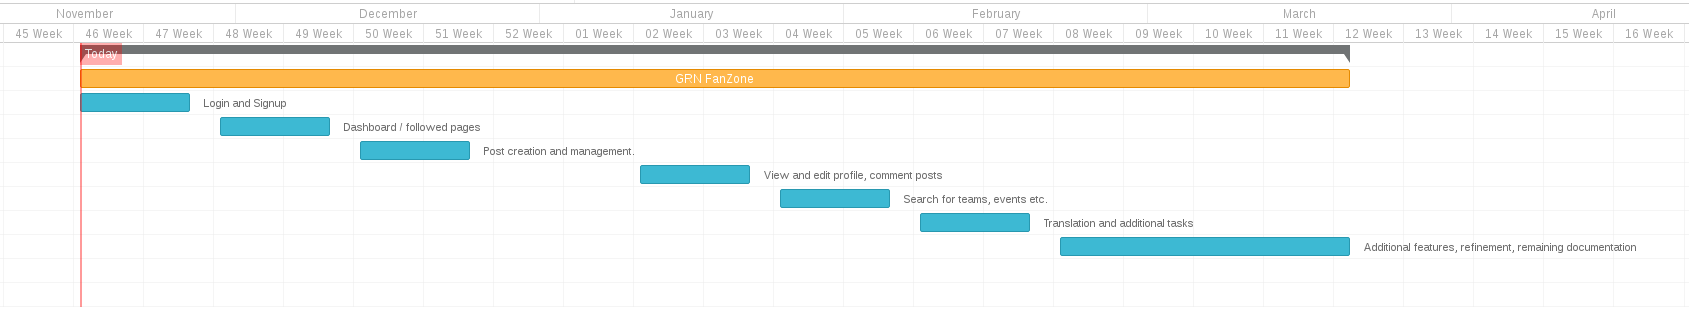
\includegraphics[width=\textwidth]{ganttchart}

"Today" on this graph refers to Monday the 14th of November 2016.


\newpage
\section{Overall description}

\subsection{Product Perspective}
The GRN FanZone will be able to source data from the GRN. This means that the data for Teams, Clubs and Players will all be managed on the GRN website, not the FanZone. 


A Firebase database will be used to store user information.


Angular 2 will be used to create a website, either in Ionic or by itself, depending on whether or not Team V is working on the app or the web app.

\subsection{Design Constraints}

There are few design constraints. The FanZone must make use of the GRN's data about Clubs, Teams and Players. This means that we have no scope to add additional information about teams. 

As we will be storing data about individuals, we will have to adhere to the Data Protection Act of 1998.


\subsection{Product Functions}

\subsubsection{Personas}


\textbf{Edinburgh Lions RFC} is an amateur league rugby club who play in the Scottish National League (BT League). They have had several successful seasons and are hoping to place highly this year after a strong start. Their fanbase has been growing fairly slowly but consistently in the past years, but engagement with supporters is low. \\


\textbf{Stewart Martins} is the \textbf{ELRFC} captain. He is 31 years old and lives in the Barnton area of Edinburgh. He usually takes on responsibility for keeping the club’s facebook page up-to-date with new games and events. His day job is at a marketing company where he works full time. He often struggles to balance the amount of time he spends marketing the club with playing and work. \\


\textbf{Sara Watson} (58) is the wife of \textbf{Jim Watson} (61), who played for the \textbf{ELRFC} when he was younger. He no longer plays rugby, but has remained involved with the club and often helps \textbf{Stewart} organise events. The two also attend games often, as their son \textbf{Tom Watson} (30) is now a second row for ELRFC. \textbf{Sara} and \textbf{Jim} both have strong social bonds with the club and many of their closest friends play there. \textbf{Sara} is now retired after working for the NHS as a nurse. \textbf{Jim} works part time at the Bank of Scotland as a teller. He worked in investment banking at Morgan Stanley until last year when he decided to “almost retire”. \\


\textbf{Struan Thomson} is a student at the University of Edinburgh. He played rugby in high school, and has continued to play at university for the 2nd XV. He is set to graduate with a 2:1 in molecular biology in May, and is now looking for a new club to play for after graduation.\\

\subsubsection{Epic}
On the 16th of November \textbf{ELRFC} has a game against the Edinburgh Academicals. This is likely to be a difficult game to win and Stewart wants to make sure that the team is in the best shape it can be in and that he can gather as big a support as he can. \\

\textbf{Stewart} has been using the GRN to help manage the team for the last year, and has found it very useful. He recently started using the GRN Fan Portal to help engage with the team’s supporters. \\

He wants to organise a game of touch rugby for the \textbf{ELRFC} with mixed teams of fans and players. This will give the team a little time off from their usually intense training schedule, and give fans a chance to get involved. \textbf{Sara} and \textbf{Jim} have also offered to bake and sell some cakes to raise funds for the team. He uses the GRN Fan Portal to announce the practice game to fans, and so that he can gauge the number of people coming. \\

At the same time, he adds the actual game to the calendar. \\

The touch rugby session is a success and lots of fans turned up. The cake sale raised around a hundred pounds which will help pay for training grounds and new kit. \textbf{Stewart} posts on the event page thanking everyone for coming along.\\

The 16th has arrived, but there’s been an issue with the Edinburgh Academicals grounds they were due to play on, so the match has to be rapidly relocated to the \textbf{ELRFC} grounds. \textbf{Stewart} quickly updates the game event with a new location, which sends an alert to everyone who said they were going, as well as the team. Everyone makes the game, and \textbf{ELRFC} wins with a last minute try. \textbf{Jim} managed to film the try on his phone, and uploads it to the team’s fan portal page so that other fans can see it. \\

\textbf{Struan}  wanted to attend the game to meet people and consider playing for them after graduation, but couldn’t because he was really hungover. He watched the try that \textbf{Jim} shared and decided he wants to contact the team to ask about playing for them. \\

\subsubsection{Epic User Stories}
\begin{itemize}

\item[1)]
As a manager/captain I want to organise a non-competitive event so that I can improve fan engagement.
\item[2)]
As fans, I want to be able to share additional information on the event page so that I can tell others my plans.
\item[3)]
As a manager/captain I want to be able to create a new fixture so that fans and players can be informed of new games.
\item[4)]
As manager/captain, I want to be able to post extra info on an event after it is over, so that fans can feel appreciated.
\item[5)]
As manager/captain, I want to be able to update details about a match, so that fans and players can be alerted.
\item[6)]
As a fan, I want to be able to share team media to the fan page.
\item[7)]
As a potential fan or player, I want to be able to discover new teams on GRN Fan Portal so that I can make decisions about joining.
\item[8)]
As a fan on the team page, I want to be able to see what other fans have posted.
\item[9)]
As a possible player, I want to be able to contact the team about joining.

\end{itemize}

\subsubsection{User Stories}

\begin{itemize}
\item[1)]
As a team manager,
I want to be able to easily ask for donations,
so that the team can afford kits, training trips, etc.

\item[2)]
As a sponsor
I want to be promoted on my sponsored player/club pages
so that I could attract new customers.

\item[3)]
As a player,
I want to be able to search for available clubs/teams,
so that I can apply and play for them.

\item[4)]
As a player
I want to be able to write status updates
so that I could share my thoughts with my supporters

\item[5)]
As a player,
I want to be able to fill out a form,
so that I can apply for sponsorship.

\item[6)]
As a club supporter,
I want to be able to donate to my team,
so that they can afford better equipment.

\item[7)]
As a club supporter
I want to have all news about my club in one place
so that I may follow my supported club easily

\item[8)]
As a rugby fan,
I want to receive notifications about matches and results,
so that I am up to date and informed.

\item[9)]
As a rugby fan,
I want to be able to search for local matches,
so that I can attend one.

\item[10)]
As an international rugby fan,
I want to be able to read about my favourite team in my native language,
so that I can easily follow their activities.

\end{itemize}

\subsection{Constraints, Assumptions and Dependencies}

\subsubsection*{Constraints}
\begin{itemize}
\item[1)]
We must finish the project by March 22nd 2017

\item[2)]
We have a development team of 5 people
\end{itemize}

\subsubsection*{Assumptions}
\begin{itemize}
\item[1)]
In a typical week, the team will have about 8 hours assigned exclusively to the project

\item[2)]
The team will have to spend their own time on the project outside of the designated times set by the University

\item[3)]
Whilst members of the team may have a primary role, they are expected to do work in other areas when they have no more specific tickets to finish
\end{itemize}

\subsubsection*{Dependencies}
\begin{itemize}
\item[1)]
The requirements document must be finished before the software begins being coded

\item[2)]
The core requirements must be completed before any extra functionality is added

\item[3)]
Tests should be written before coding starts on a module, component or directive
\end{itemize}

\newpage
\section{Wireframes}

\newpage
\subsection{Dashboard}
\fbox{ \includegraphics[width=\textwidth]{wireframe-dashboard} }

\newpage
\subsection{Team Page}
\fbox{ \includegraphics[width=\textwidth]{wireframe-team-player-page} }

\newpage
\subsection{Edit Profile}
\fbox{ \includegraphics[width=\textwidth]{wireframe-profile-edit} }

\newpage
\section{Specific requirements}
%The specific requirements for the project
\subsection{External interface requirements}

\subsubsection{User Interfaces}
\begin{itemize}
\item[1)]
There are no explicit user interface requirements set out by GRN
\end{itemize}

\subsubsection{Hardware Interfaces}
\begin{itemize}
\item[1)]
HTTP or HTTPS will be used to serve GRN FanZone to devices
\end{itemize}

\subsubsection{Software Interfaces}
\begin{itemize}
\item[1)]
Firebase will be used as a database system

\item[2)]
We will access GRN data from firebase database. We can assume it is up-to-date.


\item[3)]
We will use Angular 2 to make the website responsive
\end{itemize}

\subsubsection{Communications Interfaces}
\begin{itemize}
\item[1)]
We will target any modern web browser if making a web app
\end{itemize}

\subsection{Functional Requirements}

\subsubsection{Core Requirements}
\begin{itemize}

\item[1)]
Login as a user

\item[2)]
Signup as a user

\item[3)]
Dashboard (Lists team, club, player and fan news)

\item[4)]
Edit Profile

\item[5)]
View Profile

\item[6)]
Give instant feedback on existing posts (i.e. 'Like' or 'Tackle')

\item[7)]
Make a new post

\item[8)]
Edit an existing post

\item[9)]
Delete an existing post

\item[10)]
Comment upon an existing post

\item[11)]
Add media support to posts

\item[12)]
View a club's page

\item[13)]
View a team's page

\item[14)]
View a player's page

\item[15)]
View another follower's page

\item[16)]
Follow a club

\item[17)]
Follow a team

\item[18)]
Follow a player

\item[19)]
Follow another user

\item[20)]
Each page should be translatable into different languages

\item[20.1)]
Translation to Romanian

\item[20.2)]
Translation to Lithuanian

\item[20.3)]
Translation to Greek

\item[20.4)]
Translation to Russian

\item[20.5)]
Translation to Chinese


\end{itemize}

\subsubsection{Stretch Requirements}

\begin{itemize}

\item[1)]
Follower Groups

\item[2)]
Creation of events that users can attend

\end{itemize}

\subsection{Performance requirements}

\begin{itemize}

\item[1)]
Project must finish loading within 5 seconds on any device with a good internet connection.

\item[2)]
Project should be able to scale easily as userbase increases

\item[3)]
No transition from pages should take longer than 5 seconds

\end{itemize}

\subsection{Logical database requirement}

\begin{itemize}

\item[1)]
Database must be available constantly

\item[2)]
Database will have to store user details

\end{itemize}



\subsection{Software System attributes}

\begin{itemize}
\item[1)]
Reliable
\item[2)]
Secure
\item
Maintainable
\end{itemize}


\end{document}
